%%%%%%%%%%%%%%%%%%%%%%%%%%%%%%%%%%%%%%%%%%%%%%%%%%%%%%%%%%%%%%%%%%%%%%%%%%%%%%%%%%%%%%%%%%
\section{Results}

%%%%%%%%%%%%%%% Parameters %%%%%%%%%%%%%%%
% n_data = 20 - n_data in x and y: n_tot = 20*20
% test_size = 0.2
% noise = 0.2 - aptitude of normal distributed noise    
% data_dim = 2

%%%%%%%%%%%%%%% Part b %%%%%%%%%%%%%%%
% * Evaluate MSE up to 5.th order fro OLS. 
% * and R2 score
% * blot parameters beta
% * Your code has to include a scaling/centering:
%   XXX: not included, data is already scaled in intervall [-1, 1]

\begin{figure}[H]
    \centering
    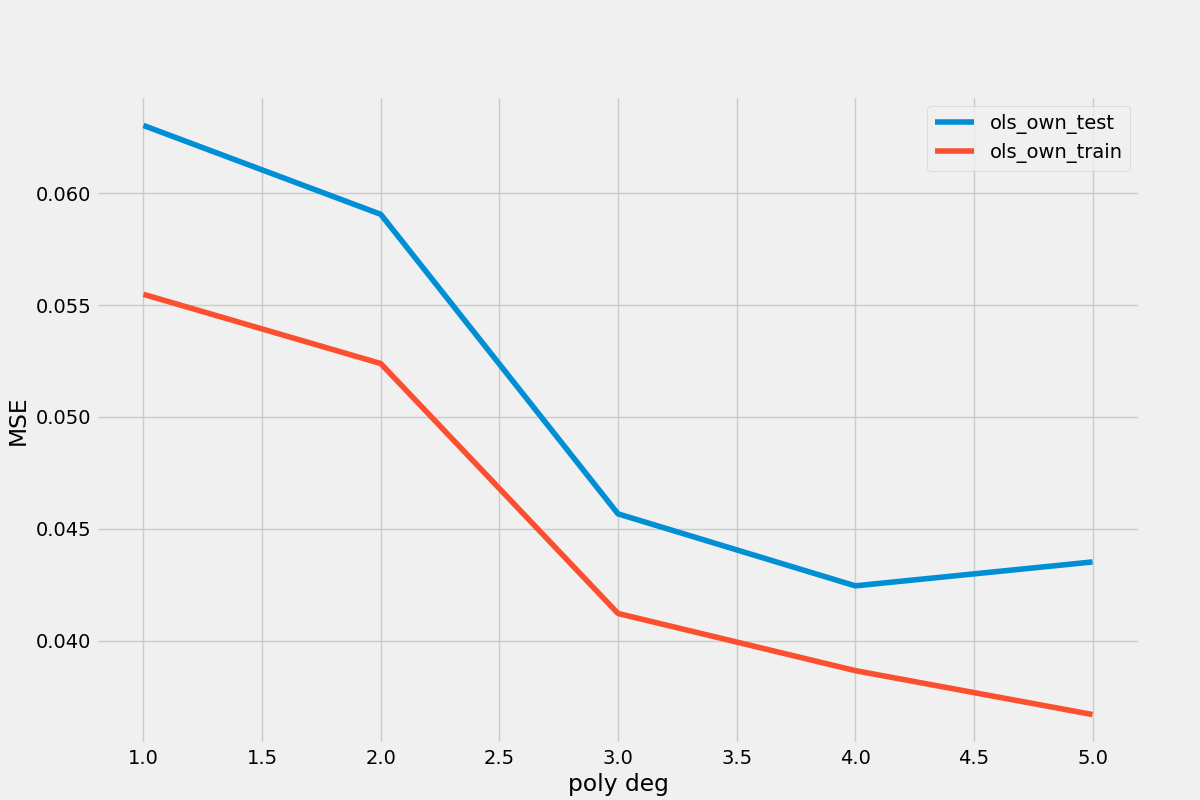
\includegraphics[width=0.8\textwidth]{Figures/b_mse.png}
\end{figure}

\begin{figure}[H]
    \centering
    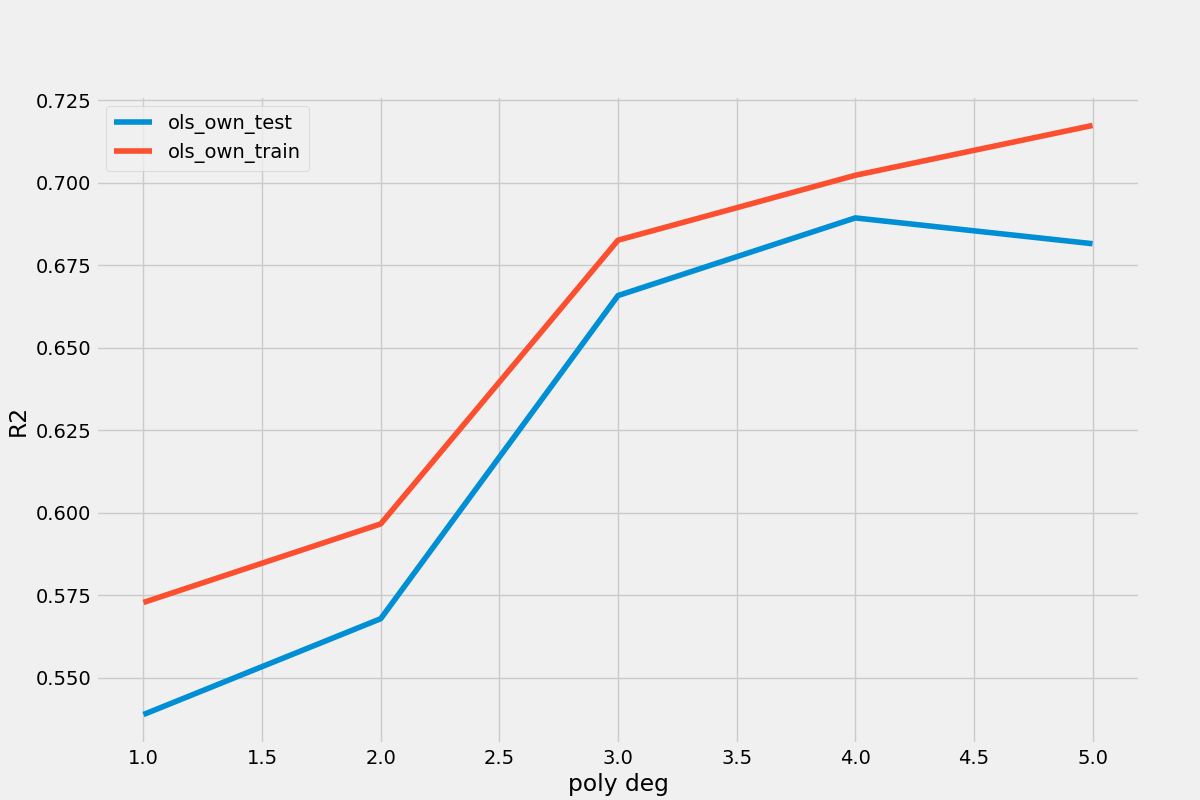
\includegraphics[width=0.8\textwidth]{Figures/b_r2.png}
\end{figure}

% TODO: error bars
\begin{figure}[H]
    \centering
    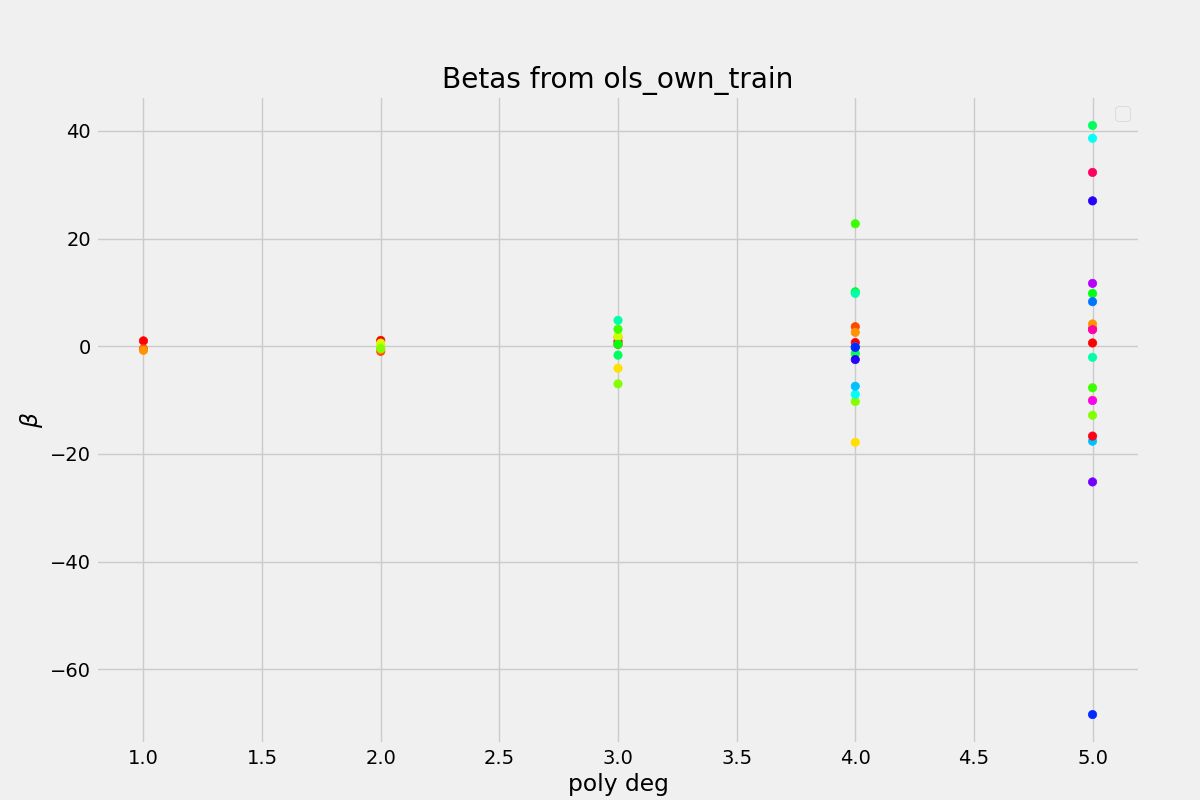
\includegraphics[width=0.8\textwidth]{Figures/b_beta.png}
\end{figure}


%%%%%%%%%%%%%%% Part c  %%%%%%%%%%%%%%%
% * Explain bias, variance, mse terms (theory) and interpretation 
% * Bias variance analysis on franke function
% * discuss in bias variance trade-off in terms of:
%   * model complexity
%   * number of data points
%   * training and test data


\begin{figure}[H]
    \centering
    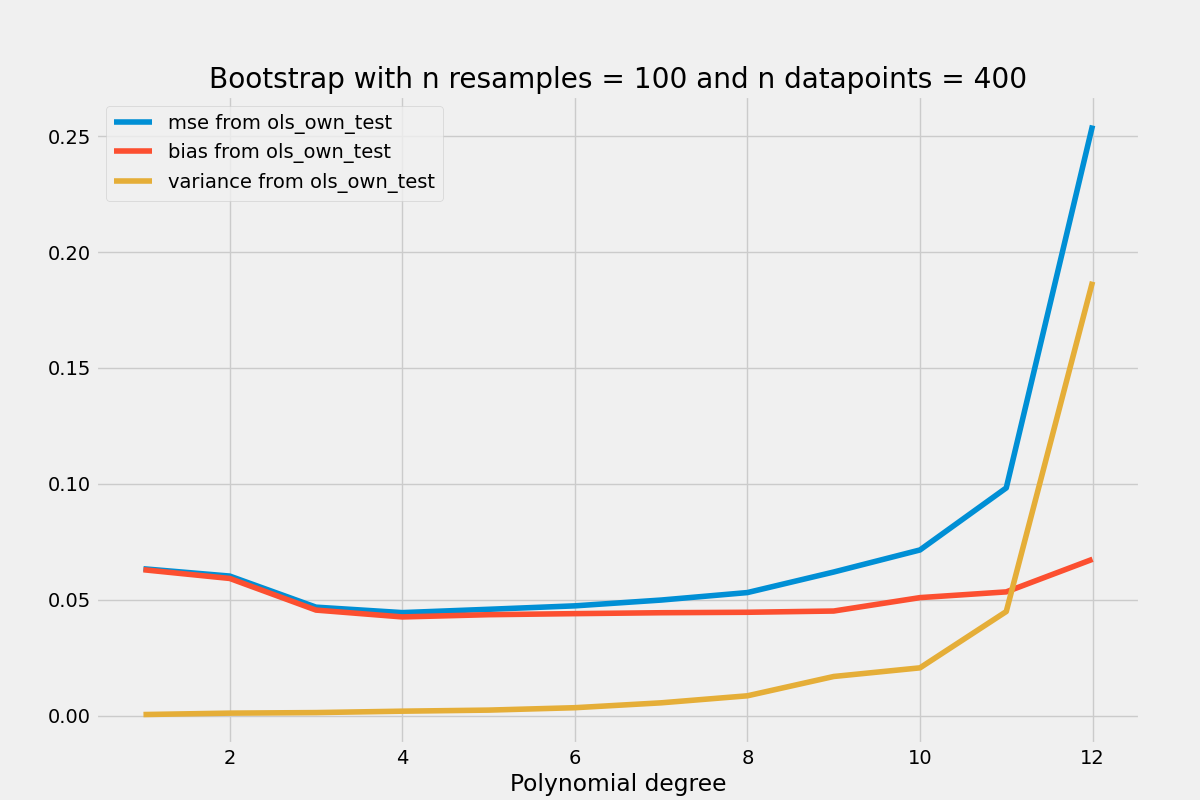
\includegraphics[width=0.8\textwidth]{Figures/c_bootstrap_ols_n_data_400.png}
\end{figure}


\begin{figure}[H]
    \centering
    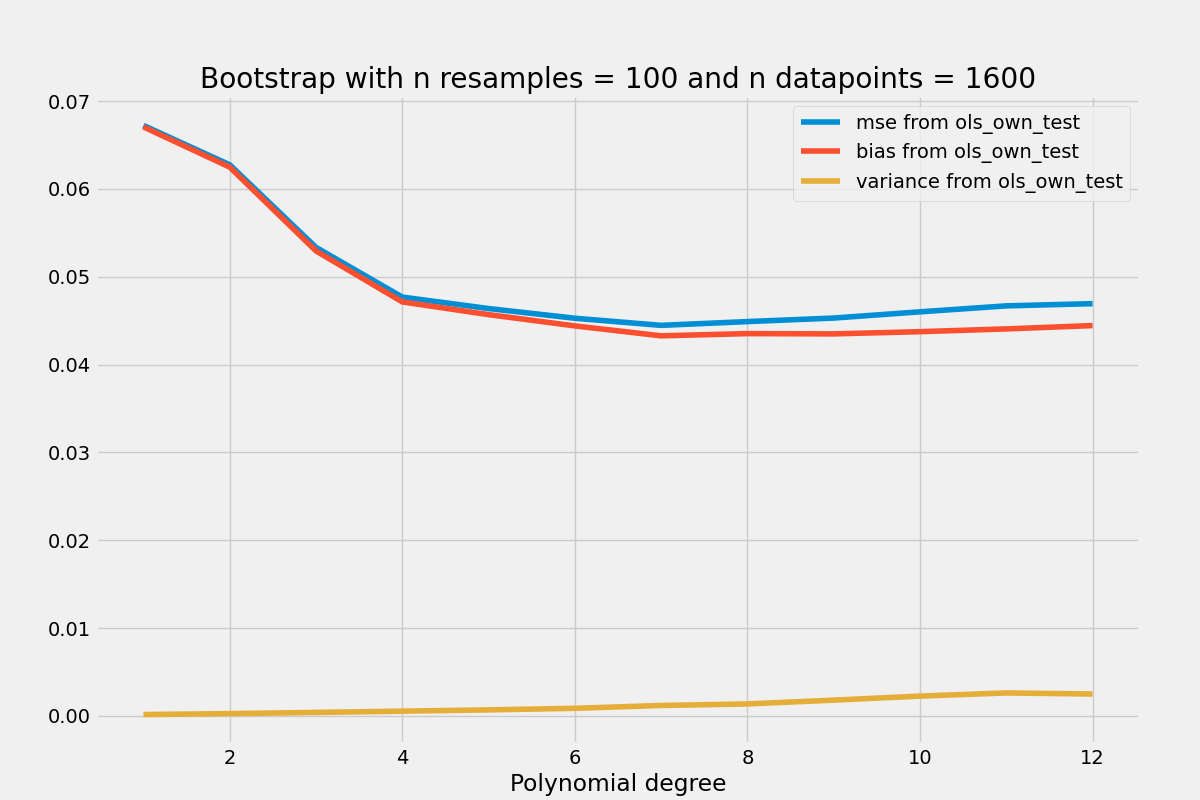
\includegraphics[width=0.8\textwidth]{Figures/c_bootstrap_ols_n_data_1600.png}
\end{figure}

% XXX: Is this expected behaviour?
\begin{figure}[H]
    \centering
    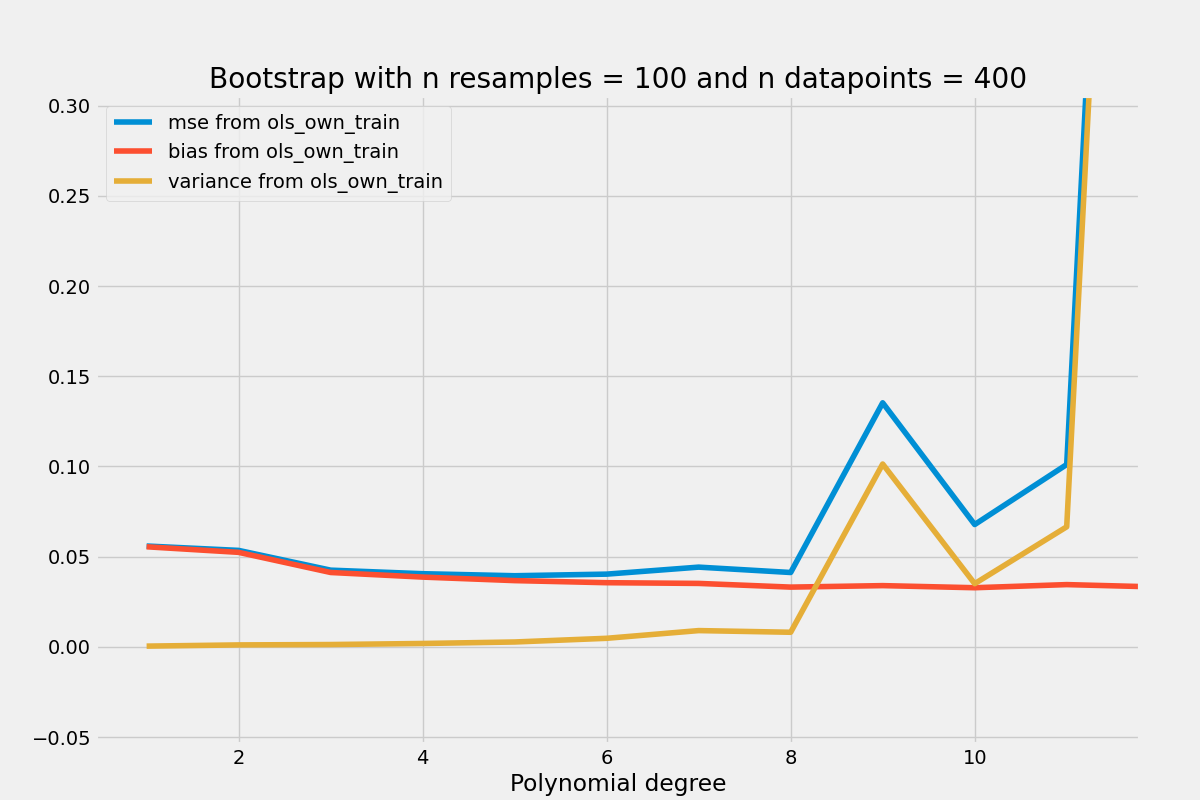
\includegraphics[width=0.8\textwidth]{Figures/c_bootstrap_ols_n_data_400_train_data.png}
\end{figure}

%%%%%%%%%%%%%%% Part d %%%%%%%%%%%%%%%
% Use k-fold and evaluate MEE on test data
% compare with bootstrap
% compare with sklearn

\begin{figure}[H]
    \centering
    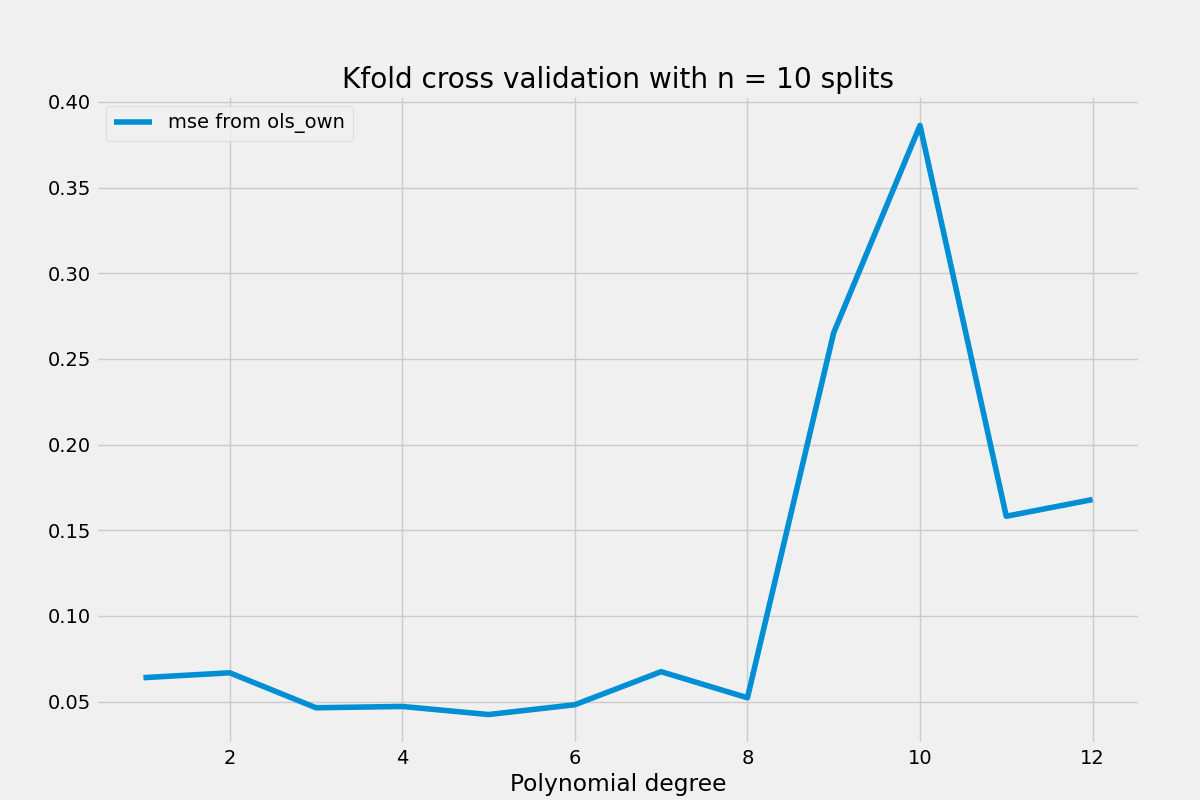
\includegraphics[width=0.8\textwidth]{Figures/d_kfold_ols_n_10.png}
\end{figure}

%%%%%%%%%%%%%%% Part e %%%%%%%%%%%%%%%
% * bootstrap analysis for ridge as in part c
% * and cross validation as in part d 
% * Compare results to those obtained in part b-d
% * study bias variance trade off for different values of lambda 

The minimum MSE from Ridge regression was found for polynomial degree of 6 with
the hyper parameter, $\lambda = 0.001$
\begin{figure}[H]
    \centering
    \caption{ridge}  
    \label{fig:e_ridge} 
    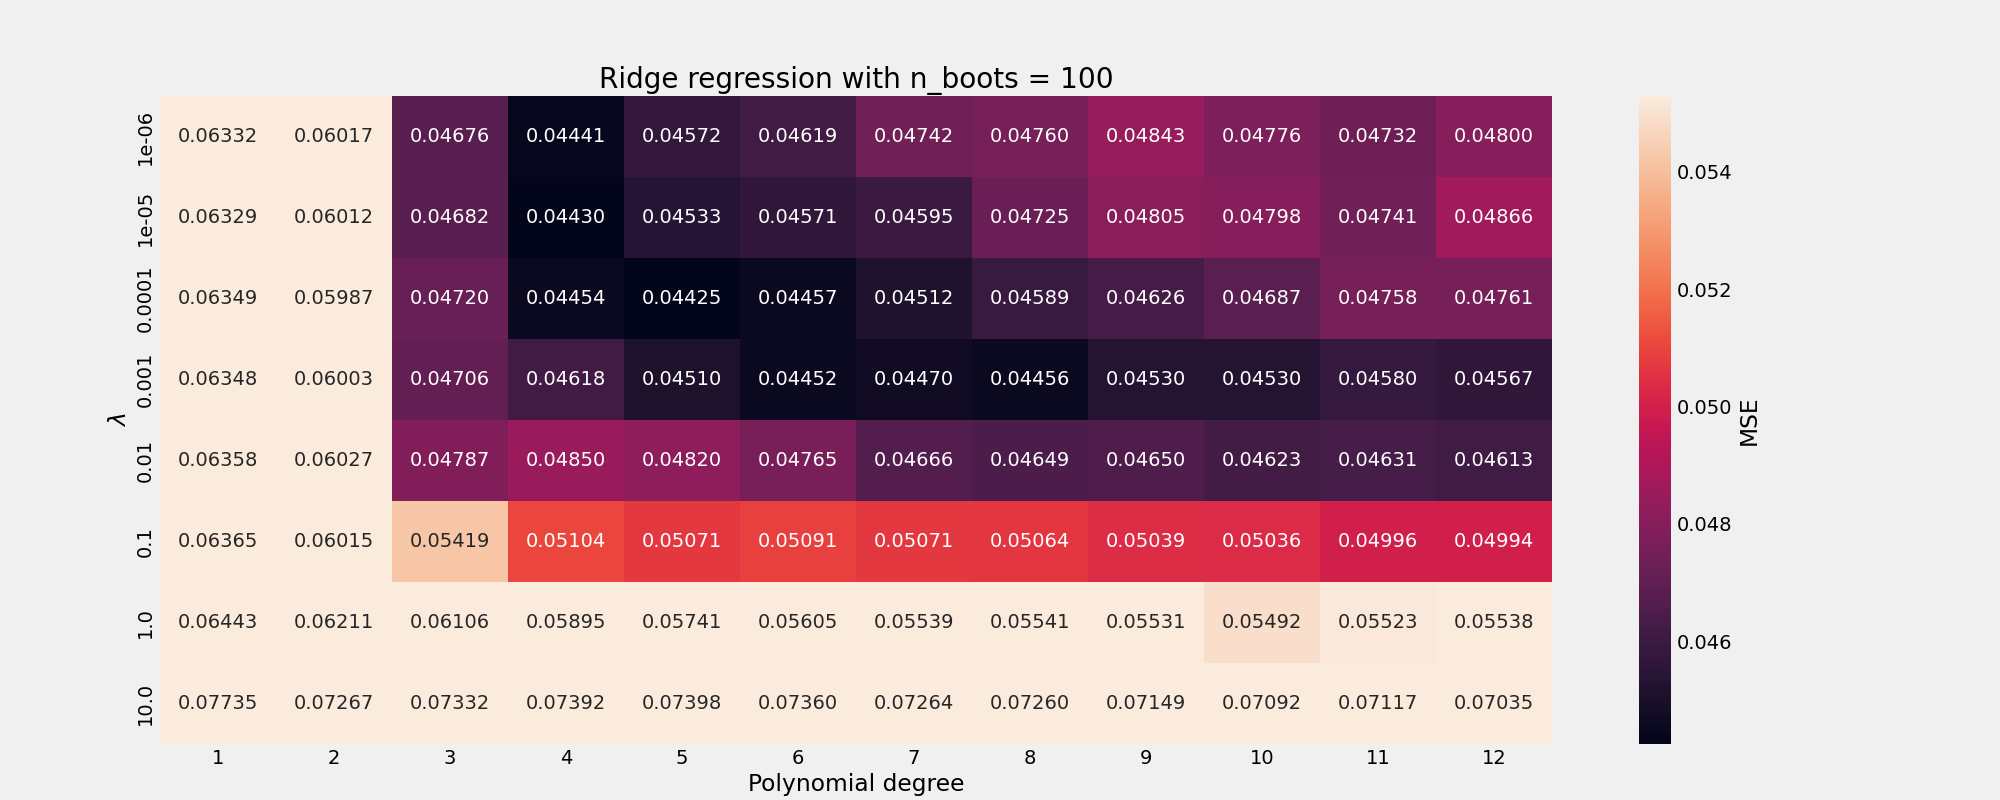
\includegraphics[width=1\textwidth]{Figures/e_ridge_n_boots_100.png}
\end{figure}

\begin{figure}[H]
    \centering
    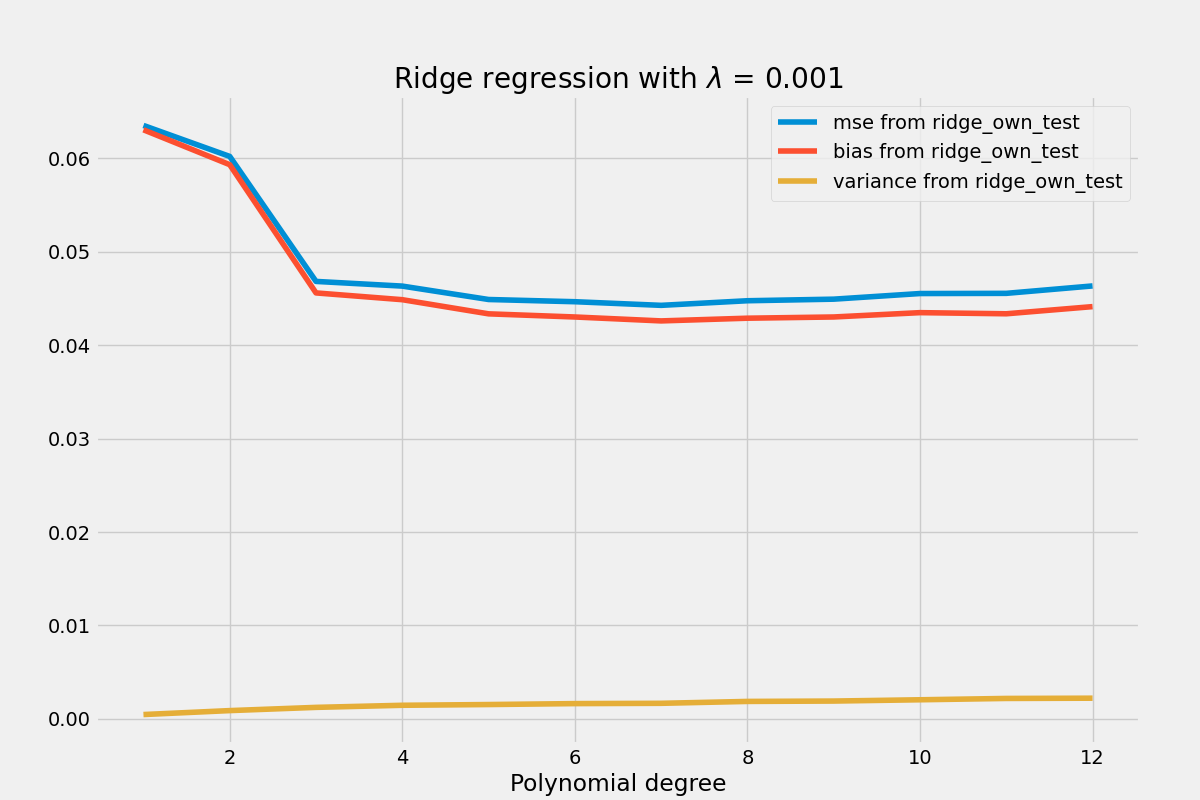
\includegraphics[width=0.8\textwidth]{Figures/e_ridge_bias_variance_lamb_0_001.png}
\end{figure}


\begin{figure}[H]
    \centering
    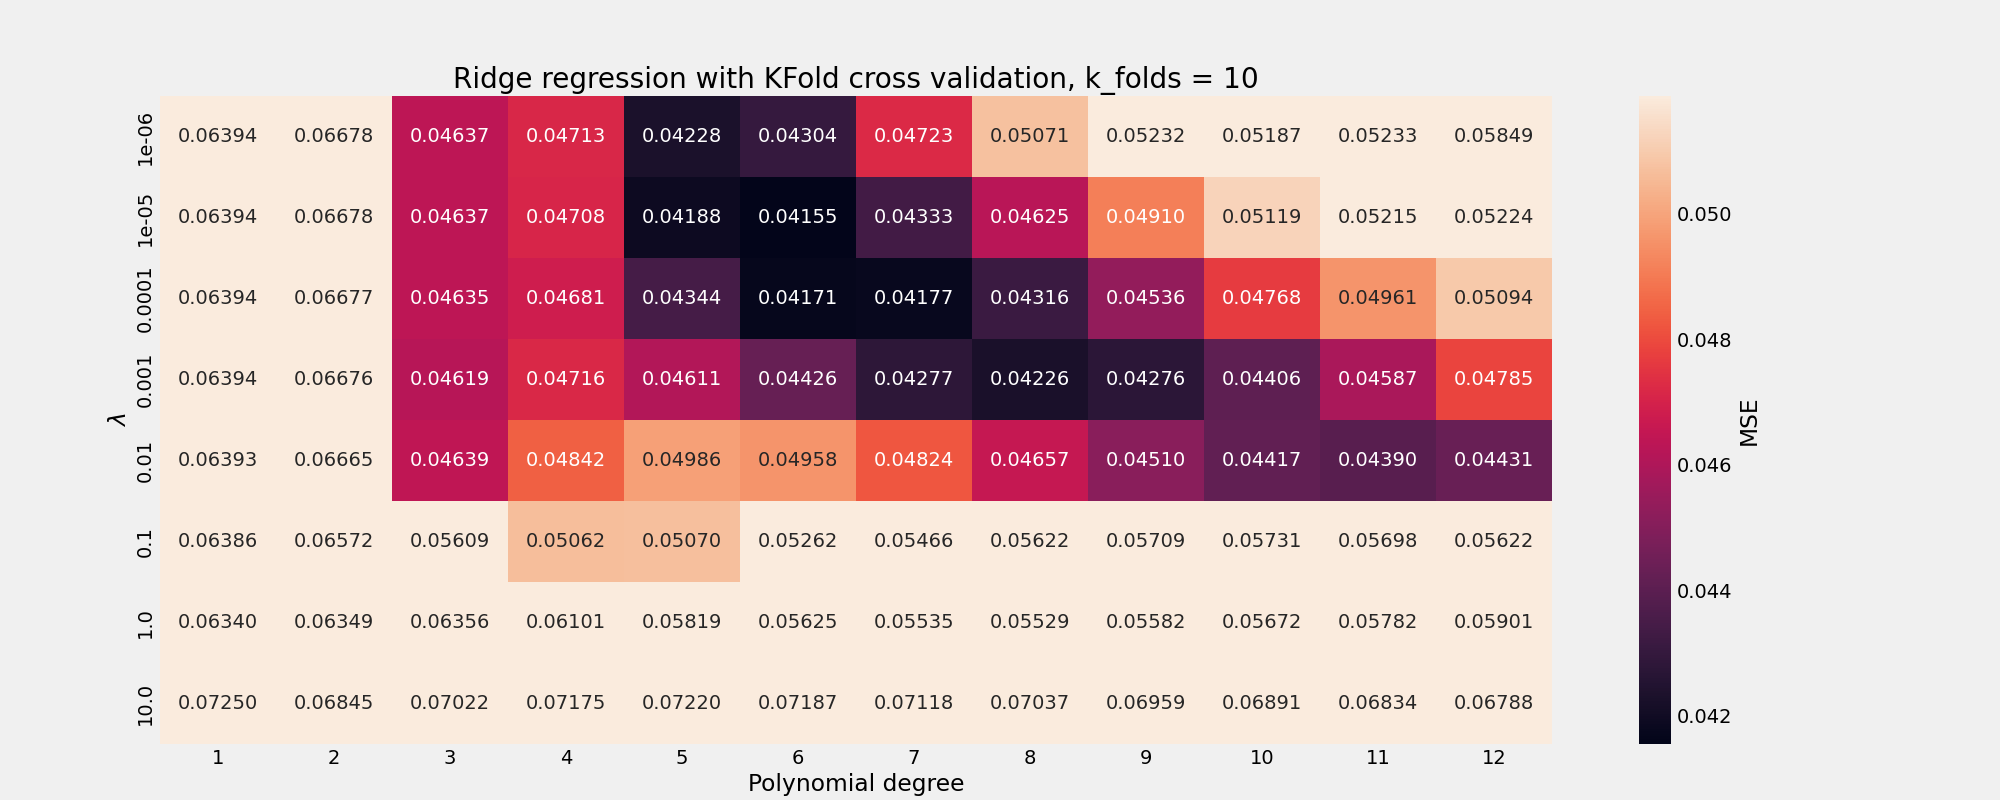
\includegraphics[width=0.8\textwidth]{Figures/e_ridge_kfold_n_10.png}
\end{figure}

%%%%%%%%%%%%%%% Part f %%%%%%%%%%%%%%%
% * Lasso regression
% * give a critical discussion of mse, ridge, lasso
% * Which model fits the data best 
% * bootstrap bias variance analysis of lasso
% * MSE analysis with kfold


\begin{figure}[H]
    \centering
    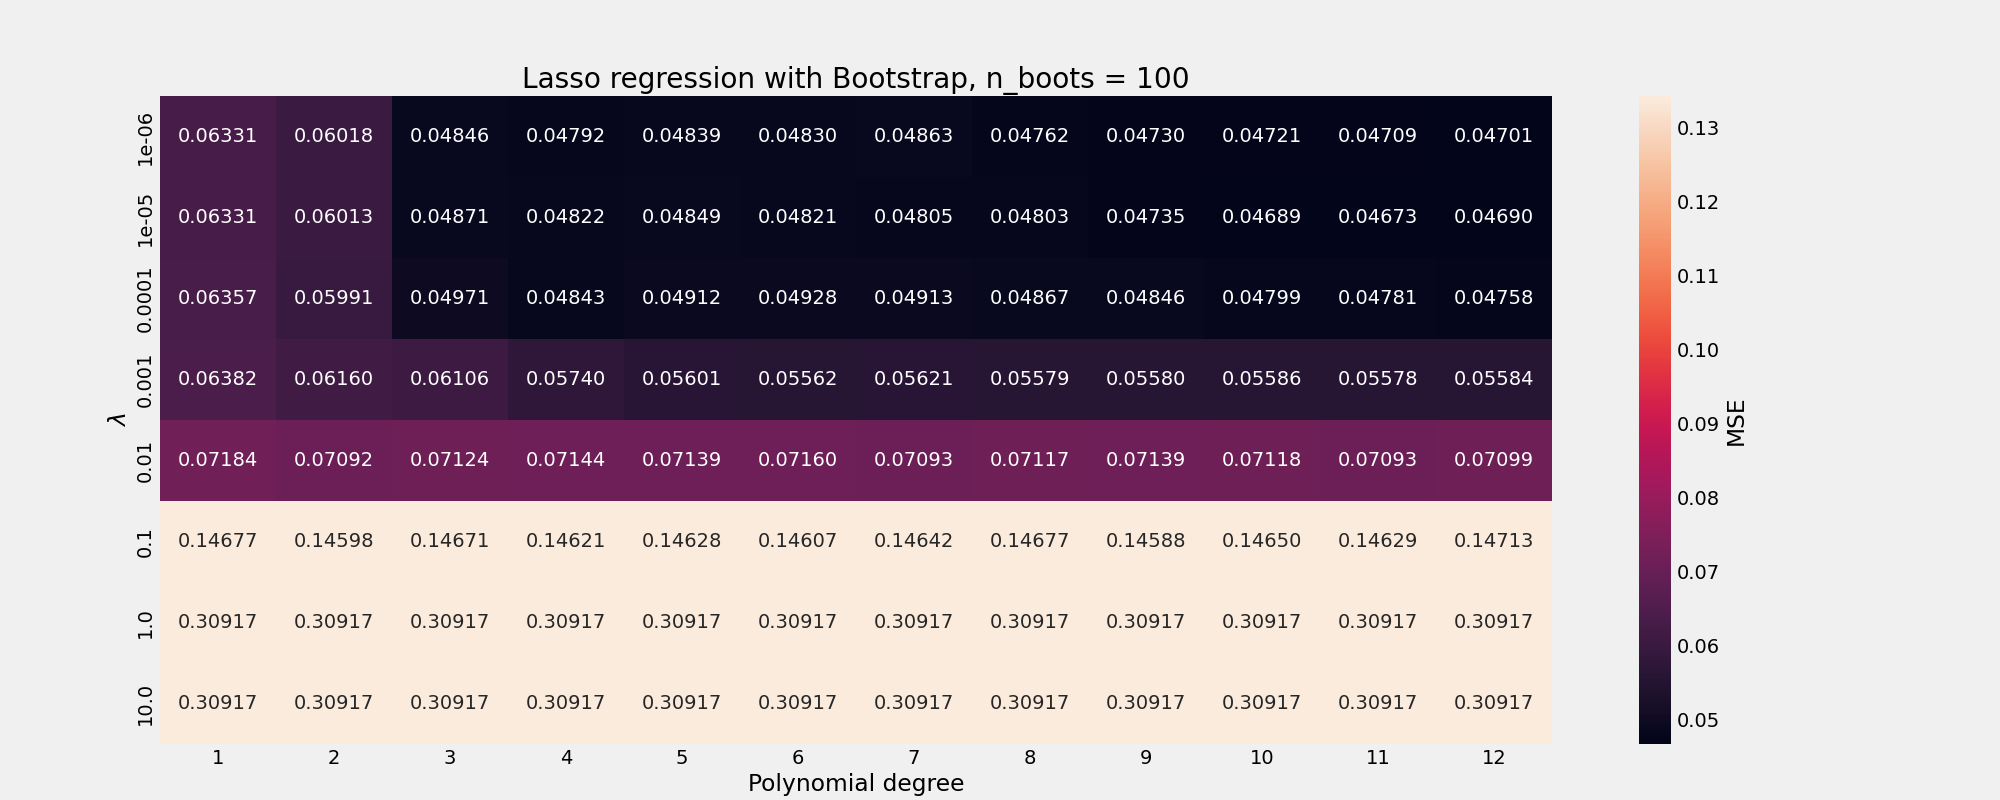
\includegraphics[width=0.8\textwidth]{Figures/f_lasso_bootstrap_n_100.png}
\end{figure}

\begin{figure}[H]
    \centering
    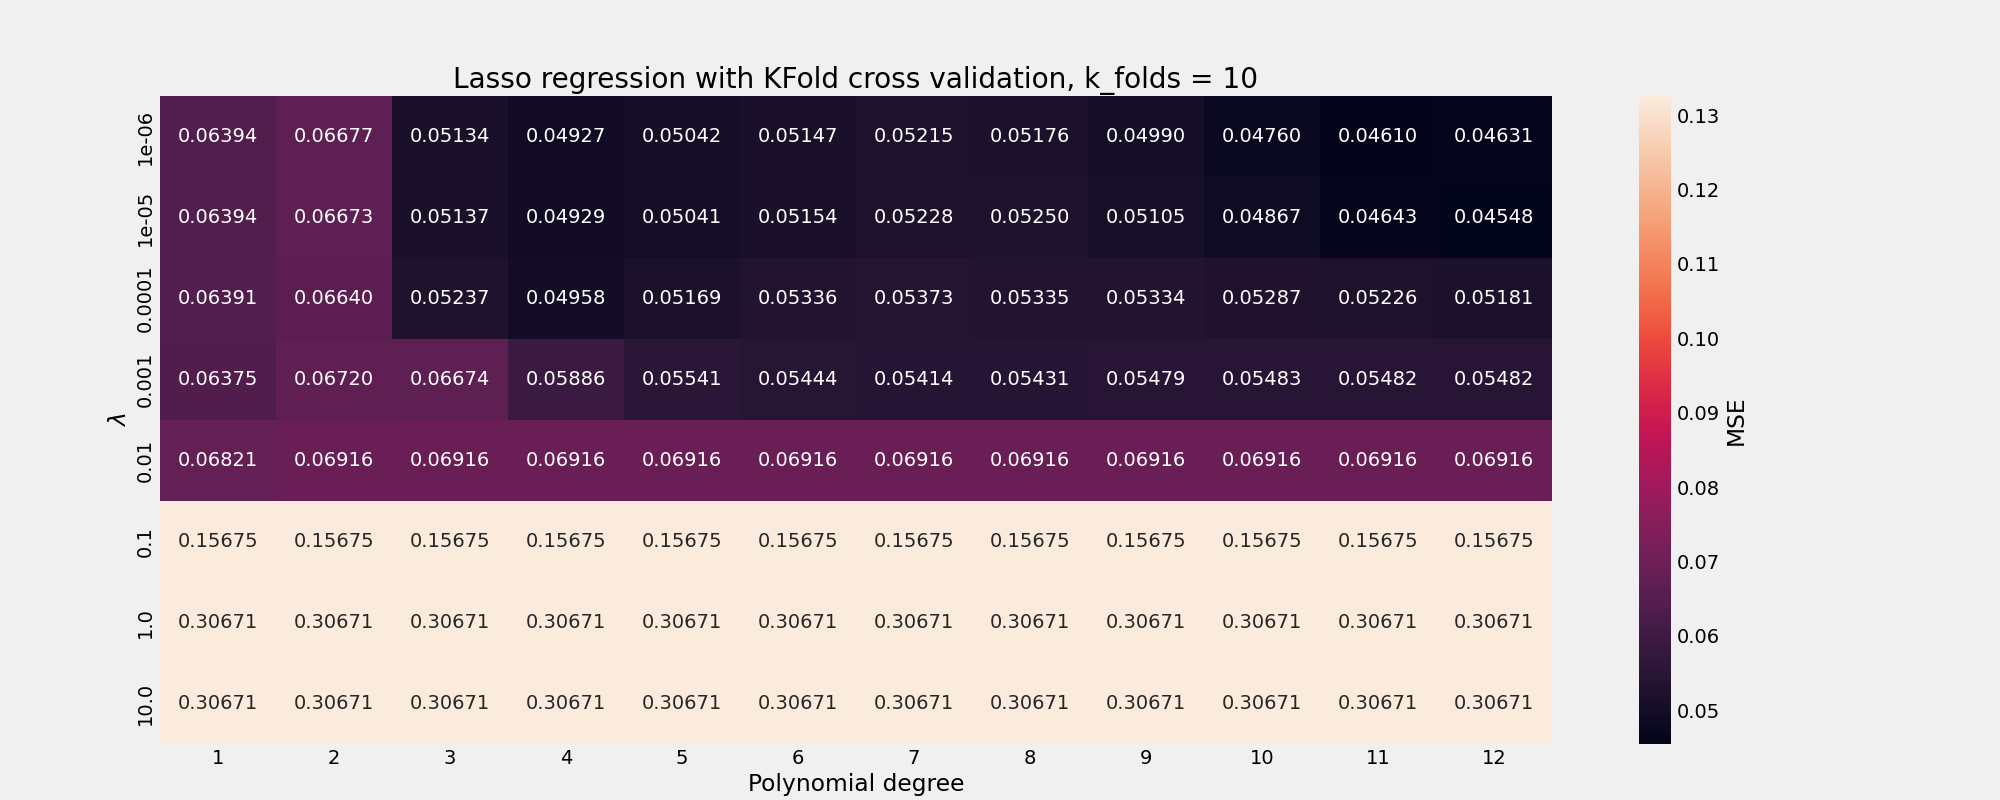
\includegraphics[width=0.8\textwidth]{Figures/f_lasso_kfold_n_10.png}
\end{figure}



% TODO: comparison of MSE for all methods
 

$R^2$ and MSE plot of OLS, Ridge and lasso
